%!TEX program = xelate
%%%%%%%%%%%%%%%%%%%%%%%%%%%%%%%%%%%%%%%%%
% Modified By Orcuslc, 2016-9-21
% Modified for Assignments
% http://github.com/orcuslc
%
% Wilson Resume/CV
% Structure Specification File
% Version 1.0 (22/1/2015)
%
% This file has been downloaded from:
% http://www.LaTeXTemplates.com
%
% License:
% CC BY-NC-SA 3.0 (http://creativecommons.org/licenses/by-nc-sa/3.0/)
%
%%%%%%%%%%%%%%%%%%%%%%%%%%%%%%%%%%%%%%%%%

%----------------------------------------------------------------------------------------
%	PACKAGES AND OTHER DOCUMENT CONFIGURATIONS
%----------------------------------------------------------------------------------------
\documentclass[10pt]{article}

\usepackage{listings}
\usepackage{xcolor}
\usepackage{amsmath,amsthm,amssymb}
\usepackage{epstopdf}
\usepackage{graphicx}
\usepackage{clrscode3e}

\DeclareGraphicsExtensions{.eps,.ps,.jpg,.bmp}


\usepackage[a4paper, hmargin=25mm, vmargin=30mm, top=20mm]{geometry} % Use A4 paper and set margins

\usepackage{fancyhdr} % Customize the header and footer

\usepackage{lastpage} % Required for calculating the number of pages in the document

\usepackage{hyperref} % Colors for links, text and headings

\setcounter{secnumdepth}{0} % Suppress section numbering

%\usepackage[proportional,scaled=1.064]{erewhon} % Use the Erewhon font
%\usepackage[erewhon,vvarbb,bigdelims]{newtxmath} % Use the Erewhon font
\usepackage[utf8]{inputenc} % Required for inputting international characters
\usepackage[T1]{fontenc} % Output font encoding for international characters

\usepackage{fontspec} % Required for specification of custom fonts
\setmainfont[Path = ./fonts/,
Extension = .otf,
BoldFont = Erewhon-Bold,
ItalicFont = Erewhon-Italic,
BoldItalicFont = Erewhon-BoldItalic,
SmallCapsFeatures = {Letters = SmallCaps}
]{Erewhon-Regular}

\usepackage{color} % Required for custom colors
\definecolor{slateblue}{rgb}{0.17,0.22,0.34}

\usepackage{sectsty} % Allows customization of titles
\sectionfont{\color{slateblue}} % Color section titles

\fancypagestyle{plain}{\fancyhf{}\cfoot{\thepage\ of \pageref{LastPage}}} % Define a custom page style
\pagestyle{plain} % Use the custom page style through the document
\renewcommand{\headrulewidth}{0pt} % Disable the default header rule
\renewcommand{\footrulewidth}{0pt} % Disable the default footer rule

\setlength\parindent{0pt} % Stop paragraph indentation

% Non-indenting itemize
\newenvironment{itemize-noindent}
{\setlength{\leftmargini}{0em}\begin{itemize}}
{\end{itemize}}

% Text width for tabbing environments
\newlength{\smallertextwidth}
\setlength{\smallertextwidth}{\textwidth}
\addtolength{\smallertextwidth}{-2cm}

\newcommand{\sqbullet}{~\vrule height .8ex width .6ex depth -.05ex} % Custom square bullet point 


\newcommand{\tbf}[1]{\textbf{#1}}
\newcommand{\tit}[1]{\textit{#1}}
\newcommand{\mbb}[1]{\mathbb{#1}}
\newcommand{\blue}[1]{\color{blue}{#1}}
\newcommand{\red}[1]{\color{red}{#1}}
\newcommand{\sblue}[1]{\color{slateblue}{#1}}
\newcommand{\n}{\\[5pt]}
\newcommand{\tr}{^\top}
\newcommand{\vt}[1]{
\Vert #1 \Vert
}
\newcommand{\bra}[5]{
#1=\left\{
\begin{aligned}
#2 ,&\quad #4 \\
#3 ,&\quad #5
\end{aligned}
\right.
}

\renewcommand{\title}[2] {
{\Huge{\color{slateblue}\textbf{#1}}}
\hfill
\LARGE{\color{slateblue}\textbf{#2}} \\[10pt]
\large{\color{slateblue}\textbf{Chuan Lu, 13300180056, chuanlu13@fudan.edu.cn}} \\[1mm]
\rule{\textwidth}{0.5mm}
}

\newcommand{\problem}[2] {
\vspace{20pt}
\LARGE{\color{slateblue}\textbf{Problem #1.}}
\vspace{2mm}
#2 \\[10pt]
}

\renewcommand{\proof}[2] {
\large{\color{slateblue}\textit{\textbf{#1.}}}
#2 \qed \\[3mm]
}

\newcommand{\solution}[2] {
\large{\color{slateblue}\textit{\textbf{#1.}}}
#2 \\[3mm]
}


\newcommand{\algorithm}[2] {
\begin{codebox}
\Procname{$\proc{Algorithm #1}$}
#2
\end{codebox}
}

\newcommand{\refgroup}[1] {
\LARGE{\color{slateblue}\textbf{Reference}} 
\begin{tabbing}
\hspace{5mm} \= \kill
#1
\end{tabbing}
}

\newcommand{\reference}[1] {
\sqbullet \ \  \large{#1} \\
}
% \newcommand{\solution}[2] {
% \LARGE{\color{slateblue}\textit{#1}}
% \ #2 \qed
% }

% \newenvironment{problem}[2][Problem]{\begin{trivlist}
% \item[\hskip \labelsep {\bfseries #1}\hskip \labelsep {\bfseries #2.}]}{\end{trivlist}}
\usepackage{epstopdf}
\usepackage{graphics}
\usepackage{subfig}
\usepackage{listings}
\lstset{
  breaklines=true,
  xleftmargin=25pt,
  xrightmargin=25pt,
  aboveskip=0pt,
  belowskip=10pt,
  basicstyle=\ttfamily,
  showstringspaces=false,
  frame=ltrb,
  tabsize=4,
  numbers=left,
  numberstyle=\small,
  numbersep=8pt,
  morekeywords={*, factorial, sum, erlang},
  keywordstyle=\color{blue!70}, commentstyle=\color{red!50!green!50!blue!50},
}
\DeclareGraphicsExtensions{.eps,.ps,.jpg,.bmp}

\begin{document}

\title{Numerical Analysis \\ Assignment 7}
\date{\today}
\author{Chuan Lu}

\maketitle

\problem{1}{Problem 3.28, Page 190.}
\solution{(a)}{
We know from the last two conditions (the first derivative),
$$
p'(x) = \frac{y_1'-y_0'}{x_1-x_0}(x-x_0)+y_0'.
$$
Integrate this polynomial we get
$$
p(x) = \frac{1}{2}\frac{y_1'-y_0'}{x_1-x_0}(x-x_0)^2+y_0'x+c.
$$
with boundary conditions we get $c = y_0-y_0'x_0$, then
$$
p(x) = y_0 + y_0'(x-x_0)\left(-\frac{(x-x_0)^2}{2(x_1-x_0)}+1\right)+y_1'\left(\frac{(x-x_0)^2}{2(x_1-x_0)}\right).
$$
}
\solution{(b)}{
We assume $p'(x_1) = y_1'$ is known. Then using Hermite interpolation we can get the fifth-order polynomial interpolation
$$
H(x) = \sum_{i=0}^{2}h_i(x) + \sum_{i=0}^{2}\tilde{h_i}(x),
$$
which satisfies
$$
\begin{aligned}
H(x_i) = y_i, ~0\le i\le 2, \\
H(x_i)' = y_i', ~0\le i\le 2.
\end{aligned}
$$
In order to get a fourth-order polynomial, we need to cancel out the coefficient of the fifth-order term, which means
$$
\sum_{i=0}^{2}(-2l_i'(x_i))\left(\frac{1}{\prod_{j\ne i}(x_i-x_j)}\right)^2y_i + \sum_{i=0}^{2}\left(\frac{1}{\prod_{j\ne i}(x_i-x_j)}\right)^2y_i' = 0.
$$
It shows
$$
\begin{aligned}
-2&\left(\frac{(x_0-x_1)+(x_0-x_2)}{(x_0-x_1)^3(x_0-x_2)^3}y_0+\frac{(x_1-x_0)+(x_1-x_2)}{(x_1-x_0)^3(x_1-x_2)^3}y_1+\frac{(x_2-x_0)+(x_2-x_1)}{(x_2-x_0)^3(x_2-x_1)^3}y_2\right) \\
+& \left(\frac{1}{(x_0-x_1)^2(x_0-x_2)^2}y_0'+\frac{1}{(x_1-x_0)^2(x_1-x_2)^2}y_1'+\frac{1}{(x_2-x_0)^2(x_2-x_1)^2}\right) = 0.
\end{aligned}
$$
with $x_i = x_0+ih$, this equation becomes
$$
y_1' = \frac{3}{4h}(y_2-y_0)-\frac{1}{4}(y_0'+y_2').
$$
Then the polynomial is 
$$
H(x) = \sum_{i=0}^{2}h_i(x)y_i + \sum_{i=0}^{2}\tilde{h_i}(x)y'_i,
$$
with
$$
\begin{aligned}
&h_i(x) = (1-2l_i'(x_i)(x-x_i))(l_i(x))^2, \\
&\tilde h_i(x) = (x-x_i)(l_i(x))^2,
\end{aligned}
$$
and $l_{i}(x)$ is the Lagrange basis.
}

\problem{2}{Problem 3.29, Page 190}
\solution{Solution}{
Assume the derivative of this quadratic polynomial is 
$$
p'(x) = a(x-x_1)+y_1'.
$$
Then integrate this we get
$$
p(x) = \frac{a}{2}(x-x_1)^2+y_1'x+c.
$$
with boundary conditions we know $a, c$ are the solutions of the linear equation system
$$
\left\{
\begin{aligned}
&\frac{(x_0-x_1)^2}{2}u+v = y_0-y_1'x_0 \\
&\frac{(x_2-x_1)^2}{2}u+v = y_0-y_1'x_2
\end{aligned}
\right.
$$
Thus the existence and uniqueness of this polynomial is equavilent to the existence and uniqueness of solution to the linear system.
Thus we know the matrix of coefficients is invertible, which means
$$
x_0 \ne x_2.
$$
Besides, in order to get a non-degenerated quadratic polynomial, the solution of $u \ne 0$. Thus
$$
y_1' \ne 0.
$$
}

\problem{3}{Problem 3.38, Page}
\solution{Solution}{
Let $k(x) = \hat{s}(x)-g(x)$, then
$$
\begin{aligned}
\int_{x_0}^{x_n}|g''(x)|^2dx &= \int_{x_0}^{x_n}|\hat{s}''(x)-k''(x)|^2dx \\
&= \int_{x_0}^{x_n}|\hat{s}''(x)|^2dx-2\int_{x_0}^{x_n}\hat{s}''(x)k''(x)dx+\int_{x_0}^{x_n}|k''(x)|^2dx.
\end{aligned}
$$
By integration by parts, 
$$
\left.\int_{x_0}^{x_n}\hat{s}''(x)k''(x)dx = \hat{s}''(x)k'(x)\right|_{x_0}^{x_n} - \int_{x_0}^{x_n}\hat{s}'''(x)k'(x)dx
$$
We know from the boundary conditions, 
$$
\hat{s}''(x_0) = \hat{s}''(x_n) = 0,
$$
thus the first term equals to $0$. Besides, since $\hat{s}(x)$ is a cubic polynomial, $\hat{s}'''(x)$ is a constant, denoted by $c$. Then 
$$
\left.\int_{x_0}^{x_n}\hat{s}'''(x)k'(x)dx = ck(x)\right|_{x_0}^{x_n} = c(k(x_n)-k(x_0)).
$$
We know from intepolation conditions that
$$
k(x_i) = \hat{s}(x_i) - g(x_i) = 0, ~0\le i\le n
$$
Thus the second term also equals to $0$. Then we know
$$
\int_{x_0}^{x_n}|g''(x)|^2dx = \int_{x_0}^{x_n}|\hat{s}''(x)|^2dx+\int_{x_0}^{x_n}|\hat{s}''(x)-g''(x)|^2dx \ge \int_{x_0}^{x_n}|\hat{s}''(x)|^2dx.
$$
}

\problem{4}{For $n = 1, \cdots, 10$, generate the Newton divided difference polynomials that interpolates $\cos(x) ~\text{for}~ x \in [0, 2\pi]$, at n equally spaced points. Create an error table.}
\solution{Solution}{
The code and result (the graph of error and table of Max error) is listed below.
}
\lstinputlisting[language = MATLAB]{newton_poly.m}
\lstinputlisting[language = MATLAB]{prob4.m}

\begin{figure}[!htb]
\centering
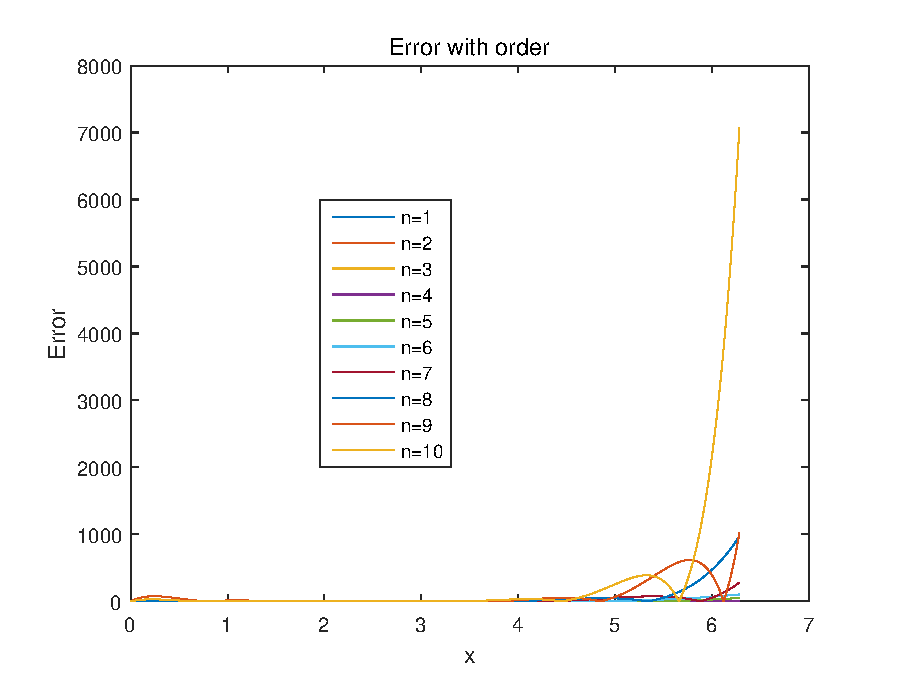
\includegraphics[width = 0.5\textwidth]{prob4.eps}
\caption{Error of interpolation with different order}
\end{figure}
\begin{lstlisting}[language = MATLAB]
>> prob4
   1.0e+03 *

    0.0020
    0.0020
    0.0040
    0.0045
    0.0520
    0.1047
    0.2818
    0.9745
    1.0237
    7.0735
\end{lstlisting}

\problem{5}{For $n = 1,\cdots, 5$, construct Hermite interpolant that interpolates $\cos(x) ~\text{for}~ x \in [0, 2\pi]$, at $n$ equally spaced points. Create an error table.
}
\solution{Solution}{
The code and result is as below. It seems Hermite intepolation is more stable then Newton intepolation.
}
\lstinputlisting[language = MATLAB]{Hermite_poly.m}
\lstinputlisting[language = MATLAB]{prob5.m}
\begin{figure}[!htb]
\centering
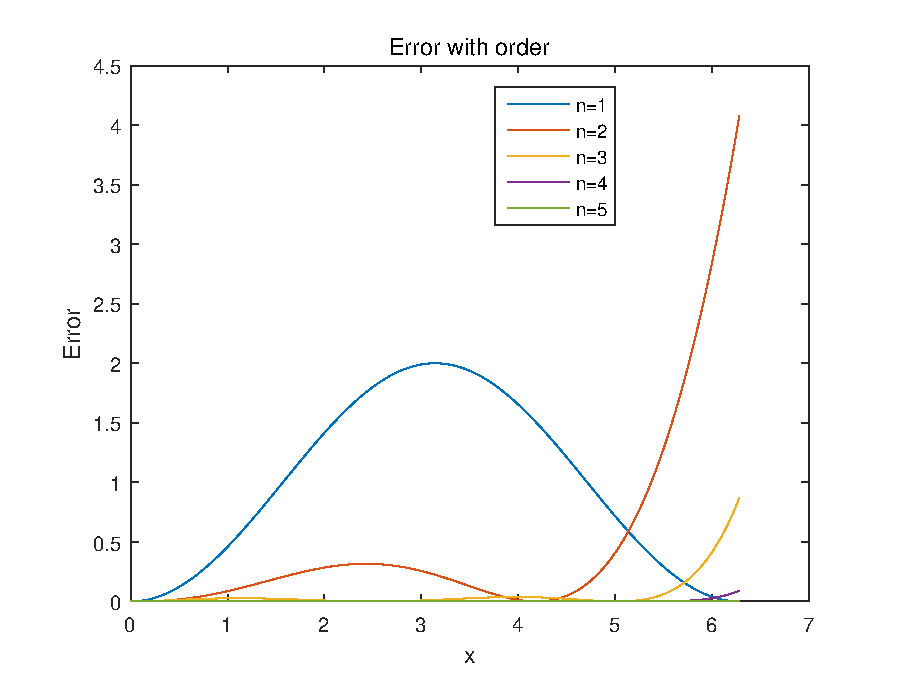
\includegraphics[width = 0.5\textwidth]{prob5.eps}
\caption{Error of Hermite interpolation with different order}
\end{figure}
\begin{lstlisting}[language = MATLAB]
>> prob5
    2.0000
    4.0801
    0.8723
    0.0900
    0.0056
\end{lstlisting}


\end{document}